%!TEX root = ../Bachelorarbeit.tex
\chapter{Überblick über die Backend-Architektur}
Im Verlauf des Projektes wurden in Zusammenarbeit mit Studierenden und den Mitarbeitern der D-School verschiedene Anforderungen an Project-Zoom als Projektverwaltungs- und Dokumentationstool entwickelt \cite{requirements}.  Aus diesen leiten sich dann die verwendeten Technologien und die umgesetzte Architektur ab. Hier aufgeführt sind nur die für diesen Teil des Projektes wichtigsten und relevanten Anforderungen. Diese beziehen sich hauptsächlich auf die Erweiterbarkeit des Systems.

\section{Systemanforderungen}
Eine wichtige Anforderung ist die übersichtliche Verwaltung der Artefakte. Hierbei sollen die von den Teams erstellten Dokumente aus der jeweiligen \gls{Box}\footnote{\url{http://box.com}} für die Studierenden in Project-Zoom zur Verfügung stehen. Diese Verfügbarkeit soll schnellstmöglich nach Hinzufügen einer neuen Datei zur \gls{Box} gegeben sein. Hierfür ist es sinnvoll ein asynchrones System zu bauen.  Neben der Anbindung von \gls{Box} ist für die Zukunft auch der Zugriff auf facebook, Dropbox und Fileshare vorgesehen. Es zeigt sich, dass ein paralleles, unabhängiges Abfragen der einzelnen Dienste notwendig ist.

Die Studierenden sollen in der Lage sein, die Anwendung auch außerhalb der D-School verwenden zu können. Dies ist wichtig, da die Studierenden meist nur zwei Tage in der Woche in der D-School verbringen. Zum Teil treffen sich die Projekt-Teilnehmer außerhalb der D-School mit Interviewpartnern und Projektpartnern, welche am Stand des Projektes interessiert sind. 

Über die Zeit verändern sich die von den Studierenden verwendeten Werkzeuge zur Dokumentation, deshalb muss das System erweitert, als auch gewartet werden können. Es ist sehr wahrscheinlich, dass ein Folgeprojekt an diesem Projekt weiterarbeiten wird. Aus diesem Grund soll das System verständlich sein und nach einer Einarbeitung von anderen Entwicklern erweitert werden können. 

Neben diesen priorisierten Anforderungen gibt es noch eine Reihe weiterer Punkte, die beim Architekturentwurf berücksichtigt werden müssen:
 
\begin{itemize}
 \item Es muss sichergestellt werden, dass kein unautorisierter Nutzer auf Daten Zugriff hat, die geschützt sind.
 \item Es sollen 100 parallele Anfragen an das Backend pro Sekunde möglich sein.
  \item Aggregierte Daten sollen nicht gelöscht werden. Es kann durchaus vorkommen, dass Daten in aggregierten Quellen nach einiger Zeit gelöscht werden müssen. Project-Zoom soll die Daten dann weiterhin vorhalten können.
\end{itemize} 

\section{Technologieauswahl}
\subsection{Webanwendung vs. native Applikation}
Bevor die Implementierung des Projektes beginnen konnte, galt es zu klären, welche Technologien verwendet werden. Eine der grundlegenden Entscheidungen war, ob eine Webanwendung oder eine native Anwendung entwickelt wird. 

Auf Grund der Anforderung der D-School, dass die Anwendung auch außerhalb der Gebäude der D-School verwendbar sein muss, liegt eine Webanwendung nahe. Hinzu kommt, dass die Projekt-Mitglieder bereits mit dem Umgang von Webseiten und deren Navigation vertraut sind. Für die Erweiterbarkeit stellt dies ebenfalls einen enormen Vorteil dar, da ein zentrales System gewartet werden kann und neue Funktionen einfach eingespielt werden können. Zudem dreht sich das Projekt um das Thema Dokumentation, bei der oft dazu geneigt wird, sie aufzuschieben. Eine Webseite senkt hier die Hemmschwelle und umgeht die Notwendigkeit einer Verteilung und Installation des Programms.

Eine Trennung der Applikation in Frontend und Backend erlaubt eine klare Funktionstrennung. Für Webapplikationen befindet sich das Backend auf Serverseite und das Frontend im Browser auf Clientseite. Die klassischen Aufgaben der beiden Teile sind:

\begin{itemize}
  \item Backend-Aufgaben:
  \begin{itemize}
    \item Sammeln und zur Verfügung stellen von Daten
    \item Kommunikation mit anderen Servern
    \item Validierung eingehender Daten vom Client
    \item Speicherung von Daten
    \item Business-Logik
  \end{itemize}

\item Frontend-Aufgaben:
  \begin{itemize}
    \item Kommunikation mit dem Backend zur Daten-Synchronisation 
\item Visualisierung der Daten
    \item Interaktion mit dem Nutzer
    \item Feedback an den Nutzer
  \end{itemize}
\end{itemize}

\subsection{Scala im Web: Play Framework}
Die Auswahl der Programmiersprache wurde vor allem von dem Gedanken geprägt, eine Sprache zu finden, die einerseits auf benötigte Bibliotheken zugreifen kann und andererseits eine kurze Einarbeitungszeit benötigt. Für die Arbeit mit Thumbnails hat sich die Bibliothek Apache Tika als besonders wertvoll erwiesen. Nähere Informationen zu dieser Bibliothek finden sich in \cite{bp-dome}. Da diese Bibliothek in Java geschrieben wurde, musste die Wahl auf eine Sprache fallen, welche in der Lage ist, Java-Bibliotheken anzusprechen. 

Um die verschiedenen Sprachen und ihr jeweiliges Webframework zu evaluieren, wurde sich mit den in Tabelle \ref{tab:FrameWorkVergleich} aufgelisteten Kombinationen näher beschäftigt. Dazu wurde von den Backend-Entwicklern jeweils eine kurze Hello-World-Anwendung aufgesetzt. Dadurch konnte festgestellt werden, ob der Arbeitsablauf, der Aufwand und der zu erzeugende Quellcode angemessen sind. Neben dieser praktischen Kurzevaluierung wurden einige Fakten zusammengetragen, um die Entscheidung zu erleichtern.

\begin{table}
  \begin{tabularx}{\textwidth}{|X|l|l|l|}
    \hline
    ~                                      & Java + Spring    & Groovy + Grails              & Scala + Play        \\\hline
    Authentifizierung                      & Ja mit Spring-WS & Ja mit Authentication Plugin & Ja mit SecureSocial \\\hline
    Json Unterstützung                     & Ja mit Jersey    & Ja                           & Ja                  \\\hline
    Vorhandene Erfahrung im Entwicklerteam & Gering           & Gut                          & Sehr Gut            \\\hline
    Dokumentation                          & Gut              & Gut                          & Gut                 \\\hline
    Asynchron                              & Nein             & Nein                         & Ja                  \\\hline
    Zustandslos                            & Nein             & Nein                         & Ja                  \\\hline
    Produktiv Einsatz                      & Einsatz          & Trial                        & Trial               \\\hline
    Wichtigkeit                            & Am wichtigsten   & Wichtig                      & Wichtiger           \\\hline
  \end{tabularx}
  \caption {Vergleich von verschiedenen Webframeworks miteinander}
  \label{tab:FrameWorkVergleich}
\end{table}

In die nähere Auswahl kamen Java, Groovy und Scala mit den jeweiligen Webframeworks Spring MVC\footnote{\url{http://www.springsource.org/features/modern-web}}, Grails\footnote{\url{http://grails.org}} und Play\footnote{\url{http://playframework.com}}. Im Gegensatz zu Spring und Grails ist Play ein zustandsloses, schlankes Framework, was eine ideale Voraussetzung für ein REST Backend darstellt. Zusätzlich spielten die persönlichen Präferenzen der Entwickler eine Rolle, die bereits Erfahrung in der Kombination Scala und Play hatten.

Scala ist eine Programmiersprache, deren Syntax stark an Java orientiert ist. Programme welche in Scala geschrieben sind, können bidirektional mit Java-Code interagieren und so auf den vollen Funktionsumfang der Java-Bibliotheken zurückgreifen. Dabei werden in der Sprache Konzepte der funktionalen mit gewohnten Elementen der objektorientierten Programmierung verknüpft. Scala eignet sich somit gut für einen allmählichen Einstieg in die funktionale Programmierung. Die Lernkurve hängt stark von den Vorkenntnissen in Java ab. Durch die starke Ähnlichkeit ist ein Umstieg einfach. Die Verwendung der hinzugekommenen, funktionalen Aspekte der Programmiersprache erfolgen nach und nach. Hier empfiehlt es sich, frei verfügbare Bücher, wie \cite{scala-by-example}, zu nutzen.

\subsection{MongoDB als Datenbanksystem}
Während der Prototypen-Phasen, in der sich die Idee der Umsetzung verfeinerte, wurde ein Datenmodell aufgestellt. Dieses Modell wird im späteren Verlauf der Arbeit näher beleuchtet. Ein wichtiger Aspekt, der für die Wahl der Datenbank entscheidend ist, sind die verschiedenen anbindbaren, externen Systeme. Das Datenmodell muss hier sicherstellen, dass Informationen, die aus allen Datenquellen verfügbar sind, einfach zugänglich sind. Gleichzeitig muss es dafür Sorge tragen, dass keine Informationen verloren gehen. Aus diesen Gründen fiel die Entscheidung auf eine NoSQL-Datenbank, welche die benötigte Flexibilität ohne großen Aufwand ermöglicht.

Neben der Open-Source Datenbank MongoDB\footnote{\url{http://mongodb.org}} stand Apache CouchDB\footnote{\url{http://couchdb.apache.org}} als Alternative zur Verfügung. Die Wahl von MongoDB als persistenten Speicher für Project-Zoom fiel vorrangig aufgrund des sehr guten Datenbank-Treibers ReactiveMongo\footnote{\url{http://reactivemongo.org}} für Scala. Dieser erlaubt komplett asynchrone Datenbankzugriffe und gliedert sich deshalb perfekt in das asynchrone Play Framework ein.

Als dokumentorientierter Datenspeicher passt MongoDB sehr gut zu einer REST-Architektur. Die Daten, welche in der Datenbank abgelegt werden, werden im Binary JSON (BSON)-Format gespeichert. Dieses BSON-Format ist eine binär encodierte Serialisierung von JSON-ähnlichen Dokumenten. BSON unterstützt die repräsentation aller Datentypen, welche auch von JSON unterstützt werden, und erlaubt zusätzlich weitere Datentypen. So wurden die JSON-Datentypen unter anderem um die Unterstützung von Binärdaten und Datumsangaben erweitert \cite{bson}. Somit ähnelt die Datenform, die auf Clientseite verarbeitet wird, dem Format der Datenspeicherung in der Datenbank. Diese Konstellation erlaubt die Implementierung einer schlanken Schicht des Datenmodells, wie sie im Abschnitt Data-centric Design \ref{sec:dcd} erklärt wird.

\subsection{Verwendete Bibliotheken}
Die umfangreichsten Bibliotheken, welche im Project-Zoom Backend Core verwendet werden, sind Akka\footnote{\url{http://akka.io}}, Play und SecureSocial\footnote{\url{http://securesocial.ws}}. Nicht hier aufgeführt ist ReactiveMongo als Datenbanktreiber. Diese Bibliothek wird im Abschnitt \ref{sec:reactive} näher erläutert. 

\paragraph{Akka} stellt die Grundlage für das Play Framework dar. Die Bibliothek ermöglicht die Nutzung verschiedenester Konzepte des asynchronen Programmierens. Das Ziel ist, das Schreiben von parallelen, fehlertoleranten und skalierbaren Anwendungen zu vereinfachen \cite{what-is-akka}. 

Die sogenannten \tete{Actors} der Bibliothek sind für dieses Projekt am relevantesten. Sie stellen eine Implementierung des Aktorenmodells dar. Aktoren sind abgeschlossene Einheiten, welche nur über Nachrichten kommunizieren. Dabei erfolgt die Abarbeitung der Nachrichten eines Aktors sequenziell, die Kommunikation mit anderen Aktoren hingegen asynchron. Dadurch können mehrere Nachrichten in unterschiedlichen Aktoren gleichzeitig abgearbeitet werden. Verschiedene Aktoren teilen sich nur über Nachrichten ausgetauschte Variablen. Damit das System also threadsicher arbeitet, müssen diese Nachrichten threadsicher sein. In Scala ist es deshalb üblich, für Nachrichten \tete{Case Classes}\footnote{\url{ http://www.scala-lang.org/node/107 }} zu verwenden. Diese sind von vornherein unveränderbar und somit threadsicher.

Neben Actors finden auch \tete{Agents} in Project-Zoom Verwendung. Ein Agent bildet eine Kapselung um einen Status. Dieser Status kann unverzüglich synchron gelesen und asynchron überschrieben werden. Bei einem Update wird dem Agent eine Funktion übergeben, welche den neuen Status des Agents berechnet. Einen Agent kann man zum Beispiel verwenden um Status zwischen verschiedenen Actors zu teilen.

\paragraph{Play Framework 2.0} ist die Weiterentwicklung  und Portierung eines früheren Java Web Frameworks nach Scala. Es ist zwar in Scala programmiert, kann aber sowohl mit Java als auch Scala als Backend Sprache verwendet werden. Play liegt ein Model-View-Controller (MVC) Architektur zugrunde. Hierbei werden in jedem \tete{Controller}\footnote{Aufgrund der allgemein üblichen Bezeichnung Model, View und Controller für die Teile einer MVC-Architekur werden diese anstatt der entsprechenden Begriffe Modell, Präsentation und Steuerung in dieser Arbeit verwendet.} sogenannte \tete{Actions} definiert und im \tete{View} verschiedene \tete{Templates} angelegt. Der Ablauf einer Anfrage an den Webserver verläuft wie folgt:

\begin{enumerate}
  \item Der standartmäßige HTTP-Router leitet die Anfrage an eine Action weiter. Diese Weiterleitung basiert auf den Routen, die in der Datei conf/routes definiert sind.
\begin{lstlisting}
GET /projects/:id controllers.ProjectController.read(id: String)
\end{lstlisting}
Eine Route besteht dabei immer aus der HTTP-Methode (GET, POST, HEAD, PUT, DELETE)\cite{play-scala-routing}, einem URI-Pattern und einer Action, die den Request beantwortet.
\item Die Action im Controller ist für die Beantwortung zuständig. Dazu können Informationen im Model abgefragt werden. Die Templates können benutzt werden, um ein dynamisches Ergebnis für den Client zu erzeugen.
\end{enumerate}

\paragraph{SecureSocial} umfasst den User-Login. Dieses Paket ist ein Authentifizierungsmodul mit Support für OAuth, OAuth2, OpenID und Username/Passwort-Authentifizierung. 

\subsection{Modularisierung}
Play erlaubt die Modularisierung des Codes in sogenannte Subprojekte. Ein solches Subprojekt ist dabei eine abgeschlossene Einheit, welche allein kompiliert, getestet und ausgeführt werden kann. Dabei können neben Play-Projekten auch Java- oder Scala-Projekte als Subprojekte verwendet werden. Die einzelnen Projekte und deren Abhängigkeiten werden in der \tete{Build.scala}-Datei angegeben.
Project-Zoom besteht aus drei verschiedenen Subprojekten:

\paragraph{common} enthält den Quelltext der sowohl von den Projekten \tete{main} als auch \tete{admin} benötigt wird. In diesem Projekt sind die Datenmodelle definiert. Weiterhin befinden sich in diesem Modul das Eventsystem, die Erweiterungen zum Datenaggregieren und zum Thumbnailgenerieren sowid die Authentifizierung.

\paragraph{main} schließt alle Controller ein, die für den normalen Nutzer ansprechbar sind. Es wurden verschiedenen Actions definiert und für die jeweiligen Sichten Templates angelegt. Der Frontend-Code, welcher näher in den Arbeiten \cite{bp-norman}, \cite{bp-tomh} und \cite{bp-anita} beschrieben ist, wird ebenfalls in diesem Projekt verwaltet.

\paragraph{admin} definiert jede Interaktion, die nur 
für privilegierte Nutzer sichtbar sein soll. Dies sorgt für eine klare Trennung zwischen User- und Admin-Anfragen und gewährleistet mehr Sicherheit. Ein weiterer Vorteil ist, dass durch das Abschalten dieses Subprojektes jedwede Admin-Aktion unterbunden werden kann.

\begin{figure}[h]  
  \centering     
  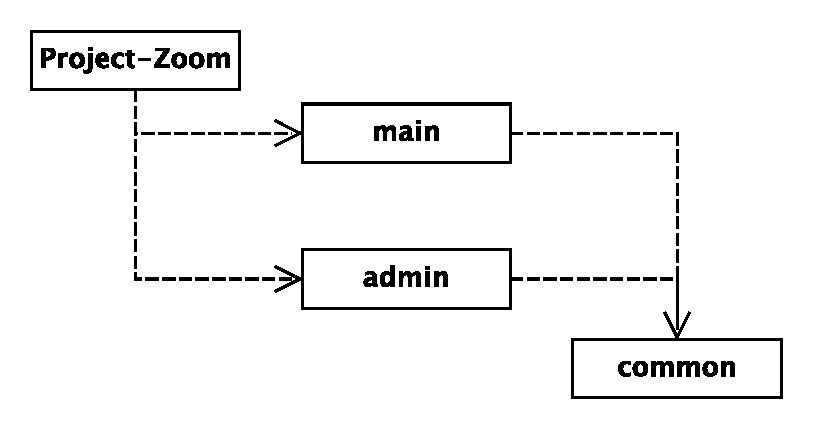
\includegraphics[width=0.8\textwidth]{img/projekte.pdf}  
   \caption{Projekte und deren Abhängigkeiten}   
  \label{fig:projects} 
\end{figure}

\FloatBarrier
In der Grafik \ref{fig:projects} sind die Abhängigkeiten der Pakte voneinander dargestellt. Das Anlegen eines Hauptprojektes, in diesem Fall Project-Zoom, erleichtert die Arbeit mit dem Gesamtprojekt. Durch die Abhängigkeit zu \tete{main} und \tete{admin} muss nur noch das Hauptprojekt kompiliert werden, denn die Abhängigkeiten werden bei Source-Code Änderungen automatisch mit kompiliert.

